\begin{figure}[h]
  \centering
  \begin{tabular}{ p{4cm} p{5cm} p{5cm} }
    \centering 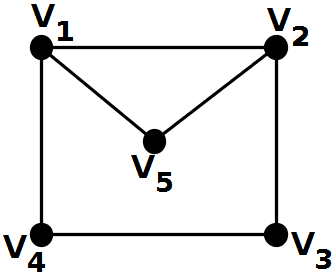
\includegraphics[width=3cm]{./img/envelope.png} & 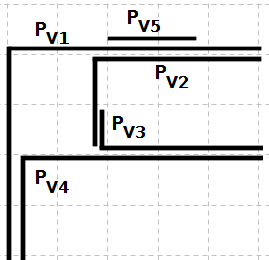
\includegraphics[width=4cm]{./img/envelopeHellyGradeTransparente.png} & 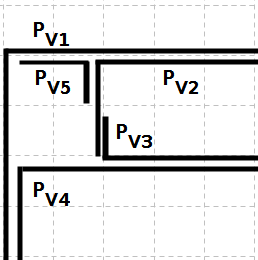
\includegraphics[width=3.8cm]{./img/envelopeNaoHellyGrade.png}
    \\
    \footnotesize \centering (a) A graph with  5 vertices. & \footnotesize(b) A $B_1$-EPG representation that satisfies the Helly property & \footnotesize (c) A $B_1$-EPG representation that does not satisfy the Helly property  \\

  \end{tabular}
\caption{A graph with 5 vertices and two of its single bend representation, the first is Helly and the second does not satisfy the Helly property.} \label{fig:envelopeRepresentacoes}
\end{figure}